\section{Architecture}

In this chapter we will detail the back end and front end aspects of the game:
how the server and the client are structured, what makes them tick and how they
communicate. We will first analyze the inner workings of the server, then those
of the client and thereafter present the communication in between.\newline

\subsection{Server}


The server was designed for relaying the information in between clients,
centralizing and managing game information - such as keeping track of the teams
and connected players. It is responsible for signalling the clients when to
enter the game and when to start playing. The first signal tells the clients
when to show the game screen and the second one tells them when to enable the
game controls.\newline

Among its roles are managing connections and resending messages - this means
receiving updates from a single client and then unicasting, multicasting or
broadcasting them. All this is done via TCP.\newline

\subsubsection{Managing connections}

For each incoming connection, the server first checks if the game is
in progress (because it is a prototype, the server only hosts one game). If
the game is indeed in progress, the incoming connection is refused. Otherwise,
it is accepted. The server holds a dictionary of connections.
The keys if the dictionary are the IP address : port pairs in the form of
InetSocketAddress object instances specific to each connection. The values
are the unique IDs of the players.\newline

Along the stages of development, connection management has been done as '1
player = 1 IP address', then '1 player = 1 IP:port pair' and ultimately as '1
player = 1 ID'. The first approach could not work for players attempting to join
the game from a subnet. The second approach created some player duplication
issues that have finally been solved with the third. This detail servers to
clarify the next detail in the process of accepting the new incoming connection:
The player connecting to the server sends a 'hello' message with his ID. If he
has no ID, he sends 'null' in the message - and the server generates a new ID
for him. In the case that the player already has an ID, the server will check if
that ID isn't already connected. If it is, the previous connection is closed and
the new one is accepted. Then, the server will confirm the ID or provide it
through the 'configuration' message - which also gives information about the
weapons, powerups and information on the players who are already connected to
the server. Once this is done, a MessageSender and a MessageReceiver object are
created and registered in specific lists. The MessageReceiver object is created
to interpret messages coming from the client and distribute them according to a
message type system. The messages can be forwarded either to the MessageSender
object, or updates entries for the HeartbeatListener - which manages all
connections. The MessageSender relays messages or constructs responses for
requests. The HeartbeatListener is an object that runs a loop and keeps a
dictionary of InetSocketAddress keys with Time objects as values. The loop
periodically checks the dictionary for signs of stale connections. If the record
for a given connection has not been updated in an inverval which spans a number
of seconds, the connection is closed.\newline

By closing the connection, we mean closing the inputs and outputs of the
communication socket, removing all communication objects and connection
record and ultimately the heartbeat records.\newline

The connection lifecycle is depicted in Figure \ref{fig:connectionLifecycle}.

\begin{figure}
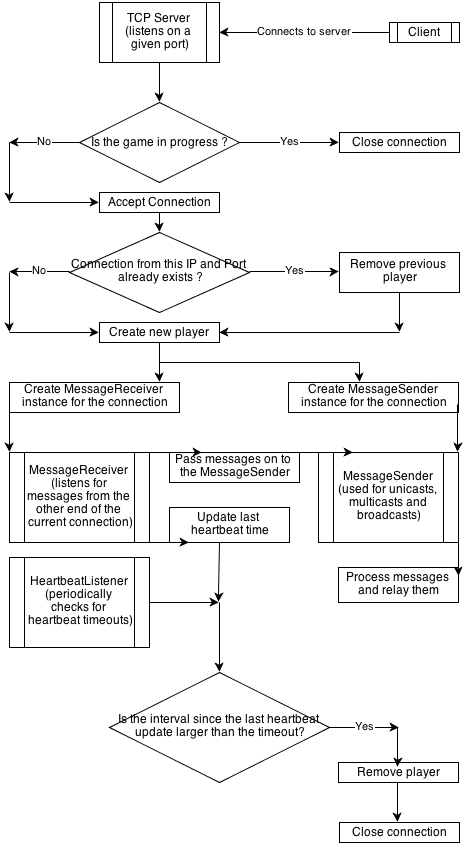
\includegraphics[height=9.00in,width=5.00in]{./images/diagrams/connection_lifecycle.png}  
\caption{\small \sl Connection lifecycle \label{fig:connectionLifecycle}}
\end{figure}

\subsubsection{Relaying messages}

The server acts as a relay, in order to lower the bandwidth and
resource consumption on the mobile clients. The messages exchanged are in
JSON format and have the following base structure: \{messageType: messageNumber,
data: \{\}\}. There are three types of messages, according to the purpose of
their usage: Administration, Lobby and In-game messages. Each of these types has
two subtypes: From Server and To Server. The server replies to or relays what
comes to other clients, according to the specifics of the messages. To this
end, the MessageReceiver checks which type the message is and if it is the case, extracts
data or sends it to the MessageSender. The MessageSender will then construct a
new message or add further fields to the existing one - for example, the
Universally Unique Identifier(UUID) of the sender. Then, according to the type
of message, it will be sent as unicast, multicast or broadcast. The unicast is
sent via the designated MessageSender. Multicasts and broadcasts are sent as
unicasts through many or all the MessageSenders available. Multicasts are, for
now, useful just for in-game messages - teams communicate within. Broadcasts are
used for most types of messages - such as position updates.\newline

\subsection{Client}

The client is the mobile application. It now works with Android versions from
2.3 up. It is structured in six modules, as seen in Figure \ref{fig:clientModules}:

\begin{figure}
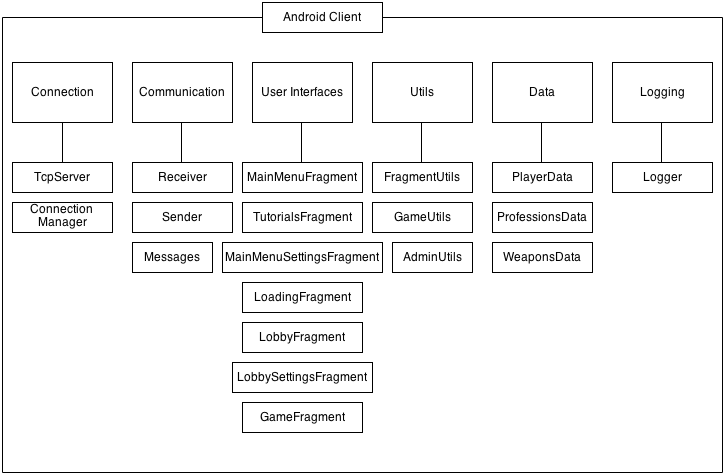
\includegraphics[height=4.08in,width=6.23in]{./images/diagrams/client_modules.png}  
\caption{\small \sl Client modules \label{fig:clientModules}}
\end{figure}

\begin{enumerate}
  \item \textbf{Connection} is responsible with managing the connections:
  starting, stopping and keeping them alive. Implicitly, it works with the
  Communication module, starting and closing the Receiver and Sender objects.
  
  \item \textbf{Communication} is responsible with receiving and
  sending messages. This implies parsing, constructing,
  interpreting, classifying messages.The messages that are to be treated are
  numbered and organized by their purpose or context, according to the
  description already given above.
  
  \item \textbf{User Interfaces} is the module that manages everything
  visual. Each screen in the UI has behind it a Fragment object. They are
  structured by purpose and interlinked. 
  
  \item \textbf{Utils} are the helper classes that provide generic methods.
  Several classes aid various aspects of the functionality of all three main
  modules: Connection, Communication and User Interfaces. For example, they are
  used to keep game state, perform various checks and activate or deactivate
  controls on the User Interfaces.
  
  \item \textbf{Storage} is composed of static classes holding
  information about the players in the game, their status, available professions
  and weapons. Also safe access to the data is provided through methods present
  in these classes. Storage also provides functionality to save data for the
  next run of the application - such as the IP and port of the server or the
  last used nickname and character type of the player. 
  
  \item \textbf{Logging} contains the Logger class, which can be used to log
  anything that would be important to be analyzed. For now, the logging module
  is responsible for storing crash dumps and data usage information in files.
\end{enumerate}

The UI of the client app is split into the 7 fragments presented under 'User
Interfaces' in Figure \ref{fig:clientModules}. When the app is run, the first
screen is the main menu. A check will be made if the prerequisits for
playing the game are met(having Google Play Services installed and the
GPS turned on). If either one is not met, a dialog will help the player
quickly get the Google Play Services or turn on the GPS. Buttons in the main
menu provide navigation to the main menu settings, tutorials or lobby(provided
there is an Internet connection). The tutorials work offline and provide some
insight on what the game is and how it is played. The settings screen is a
temporary solution for manually giving the IP address and port of the server to
which the client is to connect. The 'Connect to server' button triggers a
connection attempt. A loading screen will be briefly presented while work is
done in the background. In this case, the connection is established and 'hello'
and 'configuration' messages are exchanged by the server and client. Once this
is done, the loading screen is replaced by the Lobby screen. Here, the player
can choose between teams and edit his character details via the LobbySettings
screen. Once this is also done, the player will signal the fact that he is ready
via the 'Ready' button available on the screen. If all players are ready, the
server will send a countdown, followed by a message signalling game entry. This
is when the Lobby screen is replaced by the Game screen. The whole game UI is
available at this time, with the exception of the weapon buttons. At this point,
the server will make a check on whether the teams are far enough from each
other. When the teams get far enough from each other, the server will send the
signal to start the game. This is when the game buttons are enabled and the
virtual battle begins. The two teams will attempt to eliminate each other
through the use of virtual weapons and powerups, and strategy.\newline


\begin{figure}
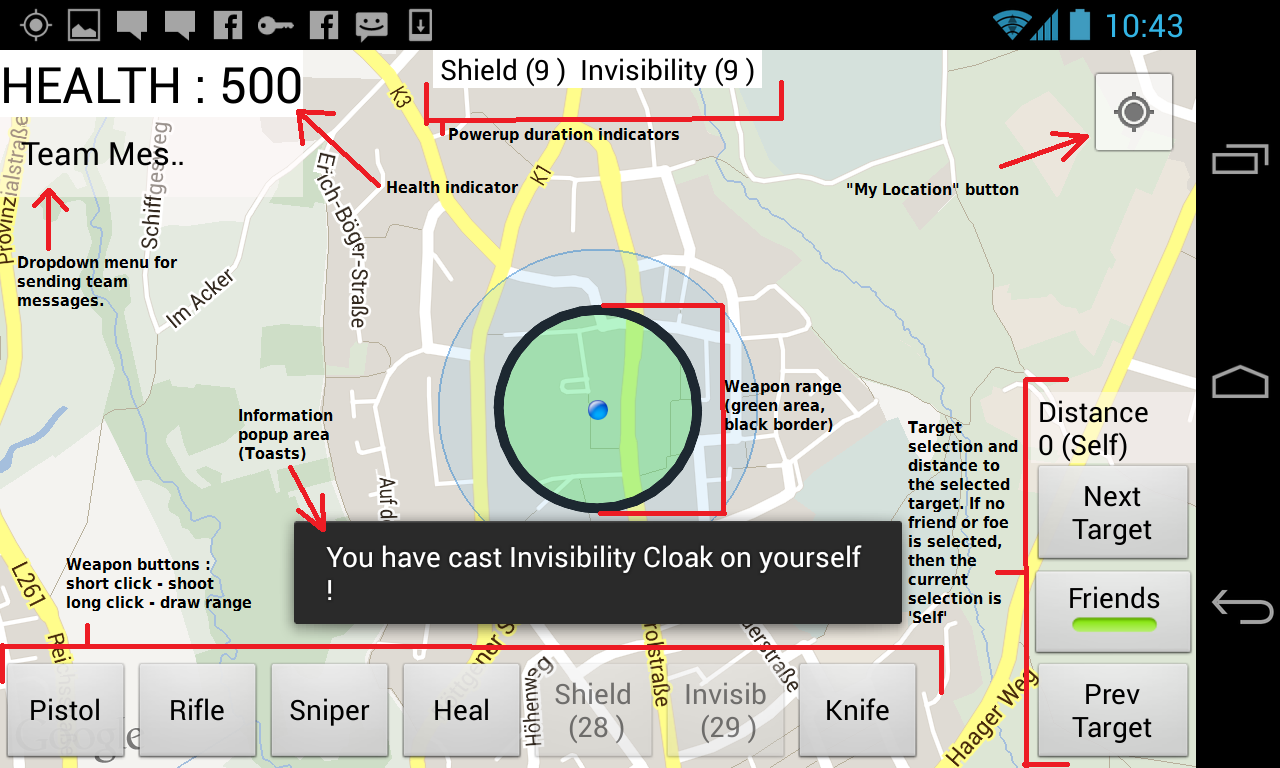
\includegraphics[height=3.5in,width=6.23in]{./images/android_screenshots/tutorial_game.png}  
\caption{\small \sl The in-game UI \label{fig:game_ui}}
\end{figure}


The in-game controls are separated in six areas, as seen in Figure\ref{fig:game_ui}:

\begin{enumerate}
  \item \textbf{The bottom area}: the Weapons: For each weapon there is a
  separate button. Each button serves three purposes: If the player presses it,
  the weapon or powerup linked to that button will shoot. If the player presses
  a weapon button for a longer time, the range of the weapon will be drawn on
  the map. Once a weapon was successfully used(on a target within its range),
  the button will be temporarily disabled and will show the weapon cooldown
  countdown.
  
  \item \textbf{The down-right corner}: The target selection buttons: The player
  can select his targets (both friends and enemies) by clicking on their
  markers on the map. As an alternative, three buttons are there to help him:
  the Friends/Enemies toggle button, with which he can choose from which
  group the selection will be made: friends or enemies. Above and below the
  toggle button are the 'Next Target' and 'Prev Target'(Previous Target)
  buttons. By pressing the 'Next Target' button, he will select the next closest
  player(If there is one selected, the next closest one will be chosen. If
  nobody is selected, the closest one will be chosen.). The 'Prev Target' button
  gets the opposite: the previous farthest friend or foe is selected, according
  to the same logic as with 'Next Target'. Above the three buttons, he can find
  a text view which shows the distance to the selected target. By clicking a
  random empty area on the screen, he will deselect whichever player was
  selected. Having no one on the screen selected is equal to having oneself
  selected - this is necessary for using powerups on oneself.
  
  \item \textbf{The top-left corner}: The health and messages buttons: The
  player's health is shown in large font. Below it, he can find the message
  selection dropdown menu. This has been arranged so that he does not waste time
  typing, but instead send critical preset messages to his team, when verbal
  communication is not possible.
  
  \item \textbf{The top-right corner}: The current position button: If the
  player presses it, the map moves to have your position in the center.
  
  \item \textbf{The top-center area}: The powerup duration views: If the player
  enables a powerup or somebody uses a powerup on him(for now, this applies only
  to the 'Shield' powerup), he will see its remaining duration of the effect
  as a countdown on the top of the screen.
  
  \item \textbf{The area above the weapon buttons}: The information area:
  Whenever the player shoots, is shot, sends or receives a message a 'Toast'
  will appear with info. The 'Toast' is an Android-specific short message that
  appears on the screen for a short time.
  
\end{enumerate}


\subsection{Communication}

Communication in between client and server is done via TCP connections that are
kept alive all along the game. The server manages a separate connection with
every client. The messages are in the JSON format and are serialized and
deserialized with the Jackson library.\newline

For each connection, the server creates a MessageSender and a MessageReceiver
objects, each acting autonomously - their lifecycle is managed by the server.
The Receiver has more responsibility, as it can close the entire connection
or call the MessageSender(or a subset of all the MessageSenders associated with
the connected clients, in the case of a broadcast or multicast) to deliver
messages.\newline

In addition to the Sender and Receiver objects, a 'heartbeat monitor' object is
running in the background and checking the liveness of all the connections. A
client sends periodic heartbeat messages to show that it is still alive. The
'heartbeat monitor' is responsible for closing the connections that have not
sent a heartbeat update in a given time frame - 3,5,10 and 15 second frames have
been tried out.\newline

As previously presented, all messages have the following JSON structure:
\{messageType: messageNumber, data: \{\}\}. We are now interested in the data
structure. The messageType is a number that both client and server recognize(as
the Messages class is present in both client and server).\newline

The Server is active in the message exchange only for the basic administration
purposes: Once a player connects, he receives a configuration json containing
the available 'weapons', 'professions' (with all their attributes) and the list
of already-connected players. It also broadcasts a message telling the existing
players that a new player has connected. When a player disconnects or is
disconnected from the server, a message telling the others that he is
disconnected is sent automatically by the server. Otherwise, the server acts as
a relay.\newline

The Messages class contains a number of inner classes, for proper
classification. We will present the structure, the message types and their
specific JSON structures within:

\begin{enumerate}
  \item \textbf{InGame.ToServer}  
  \begin{enumerate}
    \item CHANGE\_POSITION :
    \{latitude: newLatitude, longitude: newLongitude\}
    
    \item SHOOT :
    \{target: targetUUID, weapon: weaponName, (optional)timestamp: timeStamp\}
        
    \item MESSAGE\_TEAM :
    \{message : messageString\}
      
  \end{enumerate}  
  
  \item \textbf{InGame.FromServer}  
  \begin{enumerate}
    \item CHANGE\_POSITION :
    \{player: playerUUID, latitude: newLatitude, longitude: newLongitude\}
    
    \item SHOOT :
    \{player: playerUUID, target: targetUUID, weapon: weaponName, damage:    
    damageAmount, (optional)timestamp: timeStamp\}
    
    \item MESSAGE\_TEAM :
    \{player: playerUUID, message: newMessage\}
    
    \item GAME\_START :
    \{\} 
        
  \end{enumerate}  
  
  \item \textbf{Lobby.ToServer}
  
  \begin{enumerate}
    
    \item MESSAGE\_ALL :
    \{message: messageString\}
    
	\item CHANGE\_NAME :
	\{name: newName\}
			
	\item CHANGE\_TEAM :
	\{\}		
	
	\item CHANGE\_PROFESSION :
	\{profession: newProfession\}
	
	\item CHOOSE\_WEAPONS :
	this will be made available in further versions where there will be more
	weapons from which to choose
	
	\item READY :
	\{ready : true/false\}    
     
  \end{enumerate}
  
  
  \item \textbf{Lobby.FromServer}
  
  \begin{enumerate}
    	\item ENTER\_GAME :
    	\{\}
		
		\item MESSAGE\_ALL :
		\{player: playerUUID, message: messageString\}
		
		\item CHANGE\_NAME :
		\{player: playerUUID, nickname: newName\}
		
		\item CHANGE\_TEAM :
		\{player: playerUUID, team: newTeam\}
				
		\item CHANGE\_PROFESSION :
		\{player: playerUUID, profession: newProfession\}
		
		\item READY :
		\{player: playerUUID\}
										
		\item PLAYER\_JOINED :
		\{player: playerUUID, name: playerName\}
		
		\item PLAYER\_LEFT :
		\{player: playerUUID\}
			
		\item CONFIGURATION :
		A huge JSON thing that the Server composes based on a Config file and sends it
		to the client. 
		
		\item COUNTDOWN :
		\{secondsLeft: numberOfSecondsLeft\}
		
  \end{enumerate}  
  
\end{enumerate}

The communication and action flow on the server, newly joined client and
existing clients is presented in Figure\ref{fig:client_server_flow}

\begin{figure}
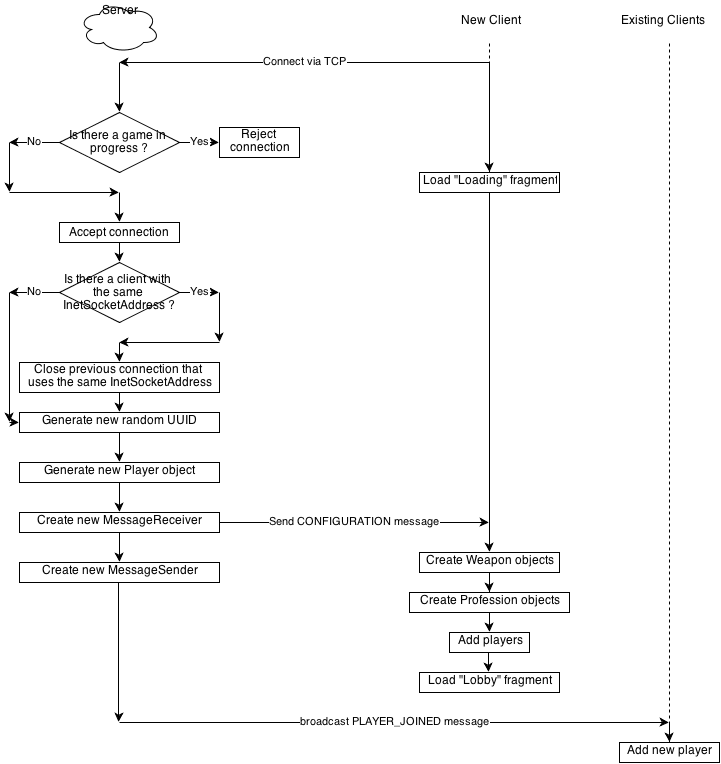
\includegraphics[height=7.665in,width=6.23in]{./images/diagrams/Client-Server.png}
\caption{\small \sl A new client joining the game
\label{fig:client_server_flow}}
\end{figure}
